\chapter{Methodology}
\label{sec:methodology}

This chapter develops PACE in full. Section~\ref{sec:m-prelim} sets up sequential
design, derives the trajectory objective that policy methods optimise, and presents
the contrastive estimators used for both training and evaluation.
Section~\ref{sec:m-saturation} diagnoses contrastive saturation (RQ1), including the
mechanisms that make it severe on biochemical systems. Section~\ref{sec:m-pace}
defines the PACE estimator and the cost it transfers (RQ2). Section~\ref{sec:m-lowess}
shows why design selection stays valid when the importance weights collapse (RQ3).
Section~\ref{sec:m-forward} gives the forward-only optimiser and its gradient
variant, Section~\ref{sec:m-eval} the evaluation protocol, and
Section~\ref{sec:m-synthesis} draws the four results together.

Everything specific to PACE is derived in this chapter. A few standard results are
stated in the text with full proofs deferred to Appendix~\ref{app:background}.

\section{Background and problem setting}
\label{sec:m-prelim}

\subsection{Sequential design and expected information gain}
\label{sec:m-bed}

A simulator generates an observation $y_t$ from unknown parameters
$\theta\in\Theta$ with prior $p(\theta)$, a design $\xi_t$, and the history
$h_{t-1}=\{(\xi_i,y_i)\}_{i=1}^{t-1}$ of past designs and outcomes (with
$h_0=\varnothing$). We assume two standard ingredients of simulation-based inference
for ODE models with explicit sensor noise: we can draw samples
$y_t\sim p(y_t\mid\theta,\xi_t,h_{t-1})$, and we can evaluate the per-step likelihood
$p(y_t\mid\theta,\xi_t,h_{t-1})$ for a simulated trajectory. The trajectory
likelihood then factorises as
$p(h_t\mid\theta)=\prod_{i=1}^{t}p(y_i\mid\theta,\xi_i,h_{i-1})$.

The value of an experiment is measured by how much it is expected to reduce
uncertainty about $\theta$. The per-step expected information gain (EIG) at $\xi_t$
given the history is the mutual information between $\theta$ and $y_t$ under the
current posterior,
\begin{equation}
\label{eq:step-eig}
I_{h_{t-1}}(\xi_t)
= \mathbb{E}_{p(\theta\mid h_{t-1})\,p(y_t\mid\theta,\xi_t,h_{t-1})}
\!\left[\log\frac{p(y_t\mid\theta,\xi_t,h_{t-1})}{p(y_t\mid\xi_t,h_{t-1})}\right],
\end{equation}
with posterior-predictive marginal
$p(y_t\mid\xi_t,h_{t-1})=\int p(y_t\mid\theta,\xi_t,h_{t-1})\,p(\theta\mid h_{t-1})\,\ud\theta$.
The two readings of this quantity are connected by Bayes' rule. Inside the expectation,
$p(y_t\mid\theta,\xi_t,h_{t-1})/p(y_t\mid\xi_t,h_{t-1})=p(\theta\mid h_t)/p(\theta\mid h_{t-1})$,
so the integrand is the log-ratio of the updated posterior $p(\theta\mid h_t)$ to the
current one. Taking the expectation over $p(\theta\mid h_{t-1})\,p(y_t\mid\theta,\xi_t,h_{t-1})$
and splitting the logarithm turns the two terms into entropies,
\begin{equation}
\label{eq:eig-entropy}
I_{h_{t-1}}(\xi_t)=H[p(\theta\mid h_{t-1})]-\mathbb{E}_{y_t}\,H[p(\theta\mid h_t)],
\end{equation}
the expected drop in posterior entropy from observing $y_t$: the first term is the current
uncertainty, the second is the uncertainty expected to remain after the experiment, and the
design that maximises one form maximises the other. The key feature for
what follows is that both the outer expectation and the denominator use the
\emph{current posterior} $p(\theta\mid h_{t-1})$, which contracts as data accumulate.
Choosing each $\xi_t$ to maximise Eq.~\eqref{eq:step-eig} is the greedy, or myopic,
design rule. PACE follows this rule; the alternative is to learn a policy that
optimises the whole trajectory at once, which we describe next because it is the
method PACE is compared against.

\subsection{From the per-step gain to the policy objective}
\label{sec:m-policy}

A design policy is a function $\pi$ that maps a history to the next design,
$\xi_t=\pi(h_{t-1})$. Running it forward produces a trajectory $h_T$ with likelihood
$p(h_T\mid\theta,\pi)=\prod_{t=1}^{T}p(y_t\mid\theta,\xi_t,h_{t-1})$. Deep Adaptive
Design (DAD) and the methods that follow it train a neural policy $\pi_\phi$ to
maximise the total information gained over the trajectory rather than greedily at
each step~\citep{foster2021deep,ivanova2021implicit}. The total objective is the sum
of the per-step gains, averaged over trajectories, and it simplifies to a single
mutual information. Summing Eq.~\eqref{eq:step-eig} in its entropy form over $t$ and
taking the expectation over trajectories,
\begin{equation}
\label{eq:traj-sum}
\mathcal{I}_T(\pi)=\mathbb{E}\!\Big[\sum_{t=1}^{T} I_{h_{t-1}}(\xi_t)\Big]
=\mathbb{E}\!\Big[\sum_{t=1}^{T}\big(H[p(\theta\mid h_{t-1})]-\mathbb{E}_{y_t}H[p(\theta\mid h_t)]\big)\Big].
\end{equation}
Each intermediate entropy $H[p(\theta\mid h_t)]$ appears twice: once as the starting
entropy of step $t{+}1$, and once inside the inner expectation of step $t$. These two
are not identical random variables, but the tower property
$\mathbb{E}[H[p(\theta\mid h_t)]]=\mathbb{E}\big[\mathbb{E}_{y_{t+1}}H[p(\theta\mid h_{t+1})]\big]$
makes them equal in expectation, so after the outer expectation the sum telescopes,
\begin{equation}
\label{eq:traj-mi}
\mathcal{I}_T(\pi)=H[p(\theta)]-\mathbb{E}\big[H[p(\theta\mid h_T)]\big]
=\mathbb{E}\!\left[\log\frac{p(h_T\mid\theta,\pi)}{p(h_T\mid\pi)}\right],
\end{equation}
the mutual information between $\theta$ and the full trajectory. This is the DAD
training objective~\citep[Theorem~1]{foster2021deep}. Casting the sequential problem
as the single quantity in Eq.~\eqref{eq:traj-mi} is what lets a policy be trained
end to end by gradient ascent, sidestepping the dynamic-programming look-ahead that a
greedy rule ignores. The same objective is used by implicit DAD for likelihood-free
models~\citep{ivanova2021implicit}, by Step-DAD which refines the policy at
deployment~\citep{hedman2025stepdad}, by a reinforcement-learning and value-based
variant~\citep{blau2022optimizing}, by amortized variants
such as vsOED and ALINE~\citep{shen2025vsoed,huang2024amortized,huang2025aline,bracher2025jadai},
and by ODE-specific specialisations~\citep{strouwen2026deep,foster2020unified}. The
obstacle, shared by all of them, is that the trajectory marginal
$p(h_T\mid\pi)=\int p(h_T\mid\theta,\pi)\,p(\theta)\,\ud\theta$ is intractable, which
forces a contrastive estimate.

\subsection{Contrastive estimators: sPCE and sNMC}
\label{sec:m-contrastive}

The contrastive construction replaces the intractable marginal with an average over
$L$ parameters drawn from the prior. With $\theta_0\sim p(\theta)$ generating the
data and contrastives $\theta_{1:L}\sim p(\theta)$, the trajectory sequential
prior-contrastive estimator is
\begin{equation}
\label{eq:traj-spce}
\mathcal{L}_T^{\mathrm{sPCE}}(\pi,L)
=\mathbb{E}\!\left[\log\frac{p(h_T\mid\theta_0,\pi)}{\frac1{L+1}\sum_{\ell=0}^{L}p(h_T\mid\theta_\ell,\pi)}\right]
\le\mathcal{I}_T(\pi),
\end{equation}
a lower bound for every $L$~\citep{foster2021deep}. DAD maximises
Eq.~\eqref{eq:traj-spce} by stochastic gradient ascent, at a cost of $O(L\cdot T)$
simulator solves per gradient step. The per-step analogue, which is the object PACE
estimates and which we use throughout for evaluation, draws $\theta_0,\theta_{1:L}$
the same way and scores
\begin{equation}
\label{eq:spce}
\mathrm{sPCE}_L(\xi_t;h_{t-1})
= \log p(y_t\mid\theta_0,\xi_t,h_{t-1})
- \log\frac{1}{L+1}\sum_{\ell=0}^{L}p(y_t\mid\theta_\ell,\xi_t,h_{t-1}).
\end{equation}
The sequential nested Monte Carlo estimator $\mathrm{sNMC}_L$ uses the same numerator
but divides the denominator sum by $L$ over the contrastives $\theta_{1:L}$ only,
excluding $\theta_0$.

These two estimators bracket the true EIG. The sPCE includes the data-generating
$\theta_0$ in its denominator. Because $\theta_0$ produced $y_t$, the term
$p(y_t\mid\theta_0,\xi_t)$ is systematically large, which inflates the denominator
and pulls the ratio down, so $\mathbb{E}[\mathrm{sPCE}_L]\le I_{h_{t-1}}(\xi_t)$. The
same inclusion caps it: the denominator is at least
$\frac{1}{L+1}p(y_t\mid\theta_0,\xi_t)$, so the ratio is at most $L+1$ and
$\mathrm{sPCE}_L\le\log(L+1)$. Equivalently, sPCE is a classification bound, since
identifying which of the $L{+}1$ exchangeable draws generated $y_t$ has success
probability at most one (Appendix~\ref{app:background}). The sNMC excludes $\theta_0$,
so its denominator is an unbiased estimate of the marginal; by Jensen's inequality
the expected log of an unbiased estimate underestimates the log of the mean, so the
log-marginal is underestimated, the log-ratio overestimated, and
$\mathbb{E}[\mathrm{sNMC}_L]\ge I_{h_{t-1}}(\xi_t)$. Both biases are $O(1/L)$, so
$[\mathrm{sPCE}_L,\mathrm{sNMC}_L]$ brackets the true EIG and tightens as $L\to\infty$.
When one method's sPCE exceeds another's sNMC, the ordering is exact regardless of
estimator bias, a fact we use throughout Chapter~\ref{sec:results}.

\subsection{Amortized neural posterior estimation}
\label{sec:m-npe}

PACE needs samples from the current posterior and the ability to evaluate their
density. Both come from a neural posterior estimator (NPE)
$q_\phi(\theta\mid h_t)\approx p(\theta\mid h_t)$, trained once per system by
simulation-based inference~\citep{cranmer2020frontier,greenberg2019automatic}. We use
a neural spline flow~\citep{durkan2019neural} because it gives fast, exact density
evaluation, which the importance weighting in Section~\ref{sec:m-pace} requires; flow
matching alternatives would require an ODE solve per density
evaluation~\citep{wildberger2024flow}. The flow is conditioned on the history through
a set-equivariant encoder and trained on randomly truncated prefixes, so one network
returns a posterior at every step $t\le T$. Because the training designs are drawn
independently of $\theta$, the network targets the correct posterior for any history,
regardless of how designs are chosen at deployment. Architecture and training are in
Appendix~\ref{app:npe}.

\section{Contrastive saturation}
\label{sec:m-saturation}

This section answers RQ1. We show that sPCE has a hard ceiling, that its gradient
vanishes as the ceiling is reached, that the budget needed to escape grows
exponentially with the information per experiment, and that biochemical systems make
this worse in three identifiable ways.

\subsection{The saturation form and the vanishing gradient}
\label{sec:m-satform}

For an observation $y_t$ generated by $\theta_0$, define the likelihood ratio of
contrastive $\ell$,
\begin{equation}
\label{eq:rratio}
r_\ell = \frac{p(y_t\mid\theta_\ell,\xi_t,h_{t-1})}{p(y_t\mid\theta_0,\xi_t,h_{t-1})}\ge 0,
\qquad \ell=1,\dots,L.
\end{equation}

\begin{lemma}[Saturation form of sPCE]
\label{lem:saturation}
The estimator in Eq.~\eqref{eq:spce} equals
$\mathrm{sPCE}_L(\xi_t;h_{t-1}) = \log(L+1) - \log\!\big(1+\sum_{\ell=1}^{L}r_\ell\big)\le\log(L+1)$,
with equality when $\sum_\ell r_\ell = 0$.
\end{lemma}
\begin{proof}
Factor $p(y_t\mid\theta_0,\xi_t,h_{t-1})$ out of the denominator sum:
$\frac{1}{L+1}\sum_{\ell=0}^{L}p(y_t\mid\theta_\ell,\xi_t,h_{t-1})
= \frac{p(y_t\mid\theta_0,\xi_t,h_{t-1})}{L+1}\big(1+\sum_{\ell=1}^{L}r_\ell\big)$.
Substituting into Eq.~\eqref{eq:spce}, $\log p(y_t\mid\theta_0,\xi_t,h_{t-1})$ cancels
and the constant $L+1$ leaves the logarithm, giving the stated form. Each $r_\ell\ge0$,
so the bound follows.
\end{proof}

Write $S=\sum_{\ell=1}^{L}r_\ell$. Saturation is the regime $S\approx 0$, where
$\mathrm{sPCE}_L\approx\log(L+1)$ for every design. The crucial point for a policy
trained by gradient ascent is that the gradient vanishes together with the value.
Only the second term of the saturation form depends on the design, so
$\nabla_{\xi_t}\mathrm{sPCE}_L=-\nabla_{\xi_t}S/(1+S)$. Writing $r_\ell=e^{\delta_\ell}$
with $\delta_\ell=\log r_\ell$ gives $\nabla_{\xi_t}r_\ell=r_\ell\nabla_{\xi_t}\log r_\ell$,
so
\begin{equation}
\label{eq:grad}
\nabla_{\xi_t}\mathrm{sPCE}_L
= -\frac{\sum_{\ell=1}^{L}r_\ell\,\nabla_{\xi_t}\log r_\ell}{1+\sum_{\ell=1}^{L}r_\ell}.
\end{equation}
The weights in the numerator are the same exponentially small ratios $r_\ell$ that
drive $S\to0$. Assume the log-likelihood-ratio surface is Lipschitz in the design,
$|\nabla_{\xi_t}\log r_\ell|\le C$, which holds for smooth simulators with Lipschitz
observation maps. Bounding the numerator term by term with the triangle inequality,
\begin{equation}
\label{eq:grad-num}
\left|\sum_{\ell=1}^{L} r_\ell\,\nabla_{\xi_t}\log r_\ell\right|
\;\le\; \sum_{\ell=1}^{L} r_\ell\,\bigl|\nabla_{\xi_t}\log r_\ell\bigr|
\;\le\; C\sum_{\ell=1}^{L} r_\ell
\;=\; C\,S ,
\end{equation}
where the first inequality is the triangle inequality, the second uses
$r_\ell\ge0$ together with the Lipschitz bound, and the last is the definition of
$S$. Dividing by the denominator $1+S$ of Eq.~\eqref{eq:grad},
\begin{equation}
\label{eq:grad-bound}
\bigl|\nabla_{\xi_t}\mathrm{sPCE}_L\bigr|
\;=\; \frac{\left|\sum_{\ell=1}^{L} r_\ell\,\nabla_{\xi_t}\log r_\ell\right|}{1+S}
\;\le\; \frac{C\,S}{1+S}
\;\xrightarrow{S\to0}\; 0 .
\end{equation}
Even without the Lipschitz bound, every term in the numerator carries the factor
$r_\ell$, which is exponentially small, so the conclusion is unchanged. This is
stronger than value saturation: not only does every design score about $\log(L+1)$,
but the gradient is near zero everywhere, so the policy receives no direction and its
parameters drift on Monte Carlo noise. Both the objective and its optimisation fail
at once.

\subsection{Why prior contrastives fail}
\label{sec:m-escape}

Saturation happens precisely when a typical prior draw assigns negligible likelihood
to the observed trajectory. To see when, compute the expected contribution of one
contrastive,
\begin{equation}
\label{eq:Er}
\mathbb{E}_{\theta_\ell\sim p(\theta)}[r_\ell]
= \frac{\int p(y_t\mid\theta,\xi_t,h_{t-1})\,p(\theta)\,\ud\theta}{p(y_t\mid\theta_0,\xi_t,h_{t-1})}
= \frac{p^{\mathrm{prior}}(y_t\mid\xi_t,h_{t-1})}{p(y_t\mid\theta_0,\xi_t,h_{t-1})},
\end{equation}
the ratio of the prior-predictive marginal to the likelihood at the truth. We
evaluate it with a Laplace approximation. Take a Gaussian prior
$p(\theta)=\mathcal N(\mu_0,\Sigma_0)$ and observation $y=\mu(\theta,\xi)+\varepsilon$
with $\varepsilon\sim\mathcal N(0,R)$, Fisher information $F=J^\top R^{-1}J$ where
$J=\partial\mu/\partial\theta|_{\theta_0}$, and posterior precision
$\Sigma_{\mathrm{post}}^{-1}=\Sigma_0^{-1}+F$. Expanding the log-likelihood to second
order about $\theta_0$ and completing the square gives a Gaussian integrand, and
integrating yields the marginal
\begin{equation}
\label{eq:laplace-marginal}
p^{\mathrm{prior}}(y\mid\xi)\approx p(y\mid\theta_0,\xi)\,p(\theta_0)\,e^{\frac12 g^\top\Sigma_{\mathrm{post}}g}\,(2\pi)^{d/2}\det(\Sigma_{\mathrm{post}})^{1/2},
\end{equation}
where $g$ is the log-posterior gradient at $\theta_0$. Dividing by
$p(y\mid\theta_0,\xi)$ and keeping the leading volume ratio,
\begin{equation}
\label{eq:escape-scale}
\mathbb{E}[r_\ell]\sim\frac{\det(\Sigma_{\mathrm{post}})^{1/2}}{\det(\Sigma_0)^{1/2}}
=\frac{1}{\det(I+\Sigma_0 F)^{1/2}}=\prod_i(1+\lambda_i)^{-1/2}=e^{-\Lambda},
\qquad \Lambda=\tfrac12\sum_i\log(1+\lambda_i),
\end{equation}
where the $\lambda_i$ are the eigenvalues of $\Sigma_0^{1/2}F\Sigma_0^{1/2}$ (similar
to $\Sigma_0 F$ and hence sharing its eigenvalues) and $\Lambda$ is the
Gaussian-linearised information gain. Appendix~\ref{app:lindley} shows that $\Lambda$ is
exactly the EIG of the linearised experiment (the Bayesian D-optimal value), so the
escape budget grows as $e^{\Lambda}=e^{\mathrm{EIG}}$. The prior-centring and mode-shift
factors omitted from Eq.~\eqref{eq:escape-scale}
contribute $O(d)$ to the exponent and do not change the exponential scaling
(Appendix~\ref{app:lindley}).

The consequence is immediate. The expected sum is $\mathbb{E}[S]=L\,e^{-\Lambda}$, so
by Markov's inequality $\Pr(S\ge1)\le L\,e^{-\Lambda}$. While $L\ll e^{\Lambda}$ the
probability that any contrastive contributes is near zero and saturation is almost
certain; escape requires $L\gtrsim e^{\Lambda}$. The contrastive budget therefore
grows exponentially with the information per experiment. We measure this with the
empirical escape threshold $L_{\mathrm{escape},50}$, the smallest $L$ at which fewer
than half of the rollouts remain within $5\%$ of the $\log(L+1)$ ceiling, evaluated
at random designs as a cheap, method-independent lower bound on the cost.
Table~\ref{tab:escape} reports it for five representative systems against the Laplace
prediction $e^{\Lambda}$.

\begin{table}[t]
\centering\small
\caption[Representative saturation thresholds]{Representative saturation thresholds,
measured at random designs, against the Laplace reference $e^{\Lambda}$. The Laplace
value matches simple systems but understates the threshold once the dynamics are
stiff or far from Gaussian, for the reasons in Section~\ref{sec:m-mechanisms}. The
full twelve-system table is in Appendix~\ref{app:lindley}.}
\label{tab:escape}
\begin{tabular}{lccrrl}
\toprule
System & $d_\theta$ & $d_\xi$ & $\Lambda$ & $e^{\Lambda}$ & $L_{\mathrm{escape},50}$ \\
\midrule
PK 1-comp & 3 & 1 & $1.02$ & $2.8$ & ${\sim}10$ \\
PI3K      & 6 & 2 & $1.49$ & $4.4$ & ${\le}10$ \\
CES       & 4 & 6 & --     & --    & ${\sim}10^4$ \\
ASM1      & 12 & 2 & --    & --    & ${\sim}10^4$ \\
SEIR R=3  & 9 & 9 & $8.64$ & $5{,}648$ & ${>}10^6$ \\
\bottomrule
\end{tabular}
\end{table}

\subsection{Mechanisms that make saturation severe}
\label{sec:m-mechanisms}

The Laplace baseline assumes a Gaussian prior, a quadratic log-likelihood, and a
unimodal posterior. Biochemical ODE systems violate all three, and the measured
threshold then exceeds $e^{\Lambda}$ by one to three orders of magnitude
(Table~\ref{tab:escape}). Three mechanisms explain this, each inflating $|\log r_\ell|$
beyond the Gaussian-quadratic prediction. They are worth stating in the main text
because they tell the experimenter, in advance, which systems will saturate.

\paragraph{Broad priors.}
Prior width enters $\Lambda$ multiplicatively through $\Sigma_0$, since the
eigenvalues $\lambda_i$ of $\Sigma_0^{1/2}F\Sigma_0^{1/2}$ scale with $\Sigma_0$.
Kinetic parameters are routinely assigned log-uniform or log-normal priors spanning
two to four orders of magnitude. A log-uniform prior over $n$ orders of magnitude has
natural-log variance $(n\ln10)^2/12\approx0.44\,n^2$, giving per-parameter prior
eigenvalues of order two to seven for $n=2$ to $4$, which inflate every $\lambda_i$
and hence $\Lambda$. Conversely tight priors ($\pm20\%$) give eigenvalues near
$0.04$, so $\lambda_i\ll1$. This is why PK 8-comp, with calibrated population priors,
has the smallest threshold in Table~\ref{tab:escape-full} despite its twenty
parameters.

\paragraph{High-dynamic-range forward maps.}
The Fisher information $F=J^\top R^{-1}J$ is large when a small parameter change
produces a large change in the output, that is when $\|J\|\gg1$. Stiff kinetics do
exactly this. A Hill function with exponent $n\ge5$ moves between its low and high
states over a narrow parameter range, so $\|J\|$ is large near the transition;
Michaelis-Menten kinetics have peak sensitivity when the substrate is near $K_m$. On
such systems a displacement of about one order of magnitude in parameter space
produces much more than one order of magnitude in observation space, and $F$ turns
this into a large $|\log r_\ell|$.

\paragraph{Non-Gaussian noise.}
The Laplace step assumed Gaussian noise, for which $\log p(y\mid\theta,\xi)$ is
exactly quadratic in the predicted mean $\mu(\theta;\xi)$. Concentration data are
usually modelled with lognormal noise instead, for which (with scale $\sigma$, per
output channel)
\begin{equation}
\label{eq:lognormal-ll}
\log p(y\mid\theta,\xi) = -\frac{1}{2\sigma^2}\bigl(\log y-\log\mu(\theta;\xi)\bigr)^2 - \log\bigl(y\,\sigma\sqrt{2\pi}\bigr).
\end{equation}
The constant $-\log(y\sigma\sqrt{2\pi})$ cancels in the log-ratio $\log r_\ell=\log
p(y\mid\theta_\ell,\xi)-\log p(y\mid\theta_0,\xi)$. Taking the expectation over
$y\sim p(y\mid\theta_0,\xi)$, write $\log y=\log\mu(\theta_0;\xi)+\eta$ with
$\mathbb{E}[\eta]=0$; the cross term in $\eta$ vanishes and, summing over output
channels $k$,
\begin{equation}
\label{eq:lognormal-gap}
\mathbb{E}_y[\log r_\ell] = -\frac{1}{2\sigma^2}\sum_k\bigl(\log\mu^{(k)}(\theta_\ell)-\log\mu^{(k)}(\theta_0)\bigr)^2 .
\end{equation}
Unlike Gaussian noise, whose gap $-\frac{1}{2}\sum_k(\mu^{(k)}(\theta_\ell)-\mu^{(k)}(\theta_0))^2/R_{kk}$
is dominated by the largest-magnitude species, the lognormal gap of
Eq.~\eqref{eq:lognormal-gap} penalises a mismatch at \emph{every} channel equally in
relative (log) terms. On stiff systems whose species span orders of magnitude, the
penalties from all channels accumulate, so $|\log r_\ell|$ is far larger than the
single dominant-species term the Gaussian baseline would predict.

Heteroscedastic Gaussian noise, with a mean-dependent scale
$\sigma(\mu)=\sqrt{(\mu\,\epsilon)^2+\nu^2}$, is worse still. A contrastive that
predicts a different order of magnitude, $\mu(\theta_\ell)\ll\mu(\theta_0)$, has a
narrow noise scale $\sigma(\mu_\ell)\ll\sigma(\mu_0)$, so the residual term
$(y-\mu_\ell)^2/\sigma(\mu_\ell)^2$ diverges because the observed
$y\approx\mu(\theta_0)$ is extreme relative to $\sigma(\mu_\ell)$. The gap again grows
super-quadratically in the mean-level displacement.

\paragraph{Combined effect.}
The three mechanisms compound through a single chain. Under the Gaussian-quadratic
baseline the gap is $|\log r_\ell|\sim(\theta_\ell-\theta_0)^\top F\,(\theta_\ell-\theta_0)$,
which decomposes as $\|\theta_\ell-\theta_0\|^2\cdot\|F\|$. Broad priors (large
$\Sigma_0$) inflate the displacement $\|\theta_\ell-\theta_0\|^2$, since prior draws
land far from $\theta_0$; high-dynamic-range maps inflate $\|F\|=\|J^\top R^{-1}J\|$
through a large Jacobian; and non-Gaussian noise then replaces the quadratic gap with
the larger forms of Eqs.~\eqref{eq:lognormal-gap} above. The amplification is
sequential: broad priors make $\|\theta_\ell-\theta_0\|$ large, high-dynamic-range
maps convert that into a large observation-space displacement, and non-Gaussian noise
converts that displacement into a more negative $\log r_\ell$ than the quadratic
approximation predicts. Systems where several mechanisms are present, such as ASM1 and
SEIR, show the largest gap between $e^{\Lambda}$ and $L_{\mathrm{escape},50}$
(Table~\ref{tab:escape}); systems with Gaussian noise (PK) track the Laplace
prediction; and systems with tight priors (PK 8-comp) have $L_{\mathrm{escape},50}\le10$
regardless of the forward map.

\begin{figure}[t]
  \centering
  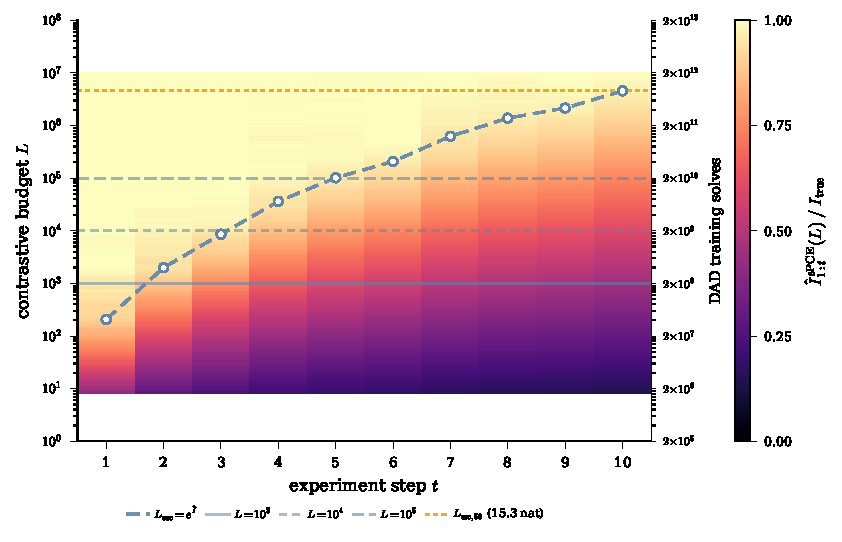
\includegraphics[width=\linewidth]{figures/fig_a1_heatmap.pdf}
  \caption[Escape threshold heatmap]{Contrastive saturation across the benchmark
  suite. Each cell shows $L_{\mathrm{escape},50}$ as a function of the contrastive
  budget $L$. Systems in which the three mechanisms compound (broad priors,
  high-dynamic-range map, non-Gaussian noise) require budgets several orders of
  magnitude above the Laplace prediction $e^{\Lambda}$.}
  \label{fig:heatmap}
\end{figure}

\section{The PACE estimator and the cost transfer}
\label{sec:m-pace}

This section answers RQ2. Prior contrastives fail because they are drawn from a
distribution that is implausible after seeing the data. PACE draws them from an
approximation to the current posterior instead, and corrects the mismatch with
importance weights.

\subsection{Definition}
\label{sec:m-pacedef}


The per-step EIG (Eq.~\eqref{eq:step-eig}) is an expectation under the current posterior of a log-ratio:
\begin{equation}
\label{eq:eig-recall}
I_{h_{t-1}}(\xi_t) = \mathbb{E}_{p(\theta\mid h_{t-1})p(y_t\mid\theta,\xi_t,h_{t-1})}
\left[\log\frac{p(y_t\mid\theta,\xi_t,h_{t-1})}{p(y_t\mid\xi_t,h_{t-1})}\right]
\end{equation}
Estimating this requires two things we do not have in closed form: samples from the current posterior $p(\theta\mid h_{t-1})$ for the outer expectation, and the posterior-predictive marginal $p(y_t\mid\xi_t,h_{t-1})=\int p(y_t\mid\theta,\xi_t,h_{t-1})p(\theta\mid h_{t-1}) d\theta$ in the denominator. The NPE gives an approximation $q_\phi(\theta\mid h_{t-1})\approx p(\theta\mid h_{t-1})$ from which we can sample and whose density we can evaluate. PACE uses importance weighting to bridge the gap. Draw $J$ particles from the NPE, $\theta_{1:J}\sim q_\phi(\theta\mid h_{t-1})$, and assign each an unnormalized importance weight
\begin{equation}
\label{eq:weights}
w_j = \frac{p(\theta_j)p(h_{t-1}\mid\theta_j)}{q_\phi(\theta_j\mid h_{t-1})}
\end{equation}
By Bayes' rule the posterior is $p(\theta_j\mid h_{t-1})=p(\theta_j)p(h_{t-1}\mid\theta_j)/p(h_{t-1})$, so $w_j$ is proportional to the posterior-to-proposal ratio $p(\theta_j\mid h_{t-1})/q_\phi(\theta_j\mid h_{t-1})$, with the unknown evidence $p(h_{t-1})$ as a constant factor across particles. This constant cancels when the weights are normalised,
\begin{equation}
\label{eq:wnorm}
\tilde w_j = \frac{w_j}{\sum_{k=1}^{J}w_k},
\end{equation}
so the normalised weights need only quantities we can compute: the prior $p(\theta_j)$, the trajectory likelihood $p(h_{t-1}\mid\theta_j)$, and the NPE density $q_\phi(\theta_j\mid h_{t-1})$. These weights turn the NPE sample into a weighted approximation of the posterior: for any function $f$, the estimate $$\sum_j\tilde w_jf(\theta_j)\to\mathbb{E}_{p(\theta\mid h_{t-1})}[f(\theta)]$$ as $J\to\infty$. This gives us both missing ingredients. For the outer expectation, the posterior average over $\theta$ is replaced by the weighted sum over particles. For the denominator, the posterior-predictive marginal is the posterior expectation of the likelihood,
\begin{equation}
\label{eq:postpred}
p(y_t\mid\xi_t,h_{t-1})=\mathbb{E}_{p(\theta\mid h_{t-1})}\big[p(y_t\mid\theta,\xi_t,h_{t-1})\big],
\end{equation}
which the weighted particles estimate as $\sum_k\tilde w_k\,p(y_t\mid\theta_k,\xi_t,h_{t-1})$. Substituting both into Eq.~\eqref{eq:eig-recall}: for each particle $\theta_j$, draw an observation $y_{t,j}\sim p(y_t\mid\theta_j,\xi_t,h_{t-1})$. The weighted average over particles approximates the outer expectation, and the weighted likelihood sum approximates the marginal denominator, giving the PACE estimator,
\begin{equation}
\label{eq:pace}
\hat I^{\mathrm{PACE}}(\xi_t;h_{t-1})
= \sum_{j=1}^{J}\tilde w_j
\left[\log p(y_{t,j}\mid\theta_j,\xi_t,h_{t-1})
- \log\sum_{k=1}^{J}\tilde w_k\,p(y_{t,j}\mid\theta_k,\xi_t,h_{t-1})\right].
\end{equation}


Each particle plays two roles: it generates an observation through $y_{t,j}$, and it acts as a weighted contrastive in the denominator for every other particle. The denominator estimates the \emph{posterior}-predictive marginal, which is the correct denominator for the per-step EIG, in contrast to the \emph{prior}-predictive marginal that the saturated sPCE denominator estimates. In implementation we average the bracket over $M$ observation draws per particle.


% PACE is built from self-normalized importance sampling, so we recall the construction before
% applying it. To estimate an expectation $\mathbb{E}_{p}[f(\theta)]$ under a target $p$ from
% which we cannot sample directly, importance sampling draws $\theta_j\sim q$ from a tractable
% proposal and reweights each draw by the ratio $w_j=p(\theta_j)/q(\theta_j)$, since
% $\mathbb{E}_{q}[w\,f]=\mathbb{E}_{p}[f]$. When the target is known only up to a normalising
% constant, as the posterior $p(\theta\mid h)\propto p(\theta)\,p(h\mid\theta)$ is, that
% constant is unknown, but it cancels if the weights are normalised to sum to one: the
% self-normalized estimate $\sum_j\tilde w_j f(\theta_j)$ with $\tilde w_j=w_j/\sum_k w_k$ is
% consistent whenever the proposal covers the target, at the price of an $O(1/J)$ bias. PACE
% applies this idea twice from a single particle set: once to retarget the NPE proposal to the
% current posterior, and once to build the posterior-predictive denominator of the per-step
% EIG from the same particles.

% Draw particles $\theta_{1:J}\sim q_\phi(\theta\mid h_{t-1})$ from the NPE and form
% self-normalized importance weights that retarget the proposal to the posterior,
% \begin{equation}
% \label{eq:weights}
% w_j = \frac{p(\theta_j)\,p(h_{t-1}\mid\theta_j)}{q_\phi(\theta_j\mid h_{t-1})},
% \qquad
% \tilde w_j = \frac{w_j}{\sum_{k=1}^{J}w_k}.
% \end{equation}
% The unnormalized weight is $w_j\propto p(\theta_j\mid h_{t-1})/q_\phi(\theta_j\mid h_{t-1})$,
% the posterior-to-proposal ratio, and the marginal $p(h_{t-1})$ cancels in the
% normalisation, so the weights need only the prior, the trajectory likelihood, and the
% NPE density. For each particle and a candidate design $\xi_t$, draw
% $y_{t,j}\sim p(y_t\mid\theta_j,\xi_t,h_{t-1})$. The PACE estimator is
% \begin{equation}
% \label{eq:pace}
% \hat I^{\mathrm{PACE}}(\xi_t;h_{t-1})
% = \sum_{j=1}^{J}\tilde w_j
% \!\left[\log p(y_{t,j}\mid\theta_j,\xi_t,h_{t-1})
% - \log\sum_{k=1}^{J}\tilde w_k\,p(y_{t,j}\mid\theta_k,\xi_t,h_{t-1})\right].
% \end{equation}
% Each particle plays two roles: it generates an observation through $y_{t,j}$, and it
% acts as a weighted contrastive in the denominator for every other particle. The
% denominator is a self-normalized estimate of the posterior-predictive marginal
% $p(y_t\mid\xi_t,h_{t-1})$, which is the correct denominator for the per-step EIG in
% Eq.~\eqref{eq:step-eig}, in contrast to the prior-predictive marginal that the
% saturated sPCE denominator estimates. In implementation we average the bracket over
% $M$ observation draws per particle. Algebraically Eq.~\eqref{eq:pace} is the per-step
% instance of the importance-weighted contrastive bound whose trajectory form appears
% in the appendices of \citet{foster2021deep} and \citet{ivanova2021implicit}; the
% difference is that $q_\phi$ is trained once by SBI rather than jointly with a policy.

\begin{theorem}[Consistency]
\label{thm:consistency}
If $q_\phi(\cdot\mid h_{t-1})$ supports $p(\cdot\mid h_{t-1})$, the chi-square
divergence $\chi^2(p(\cdot\mid h_{t-1})\,\|\,q_\phi(\cdot\mid h_{t-1}))$ is finite, and
the per-step EIG is finite, then $\hat I^{\mathrm{PACE}}(\xi_t;h_{t-1})\to I_{h_{t-1}}(\xi_t)$
almost surely as $J\to\infty$, with bias $O(1/J)$.
\end{theorem}

This is the standard two-stage self-normalized importance sampling argument: support
inclusion makes the weighted numerator and denominator converge to the posterior
expectations, and finite chi-square gives the $O(1/J)$ rate through the SNIS central
limit theorem (Appendix~\ref{app:pace}). The estimator is decoupled by construction.
The NPE is trained by minimising $-\mathbb{E}_{p(\theta)p(h\mid\theta)}[\log q_\phi(\theta\mid h)]$,
whose gradient is informative no matter how informative the system is, and is then
frozen. This breaks the circular dependence in which a policy and its contrastive
proposal are trained together and both lose signal once sPCE saturates.

\subsection{Relation to ACE, sACE, and sLACE}
\label{sec:m-relation}

The estimator in Eq.~\eqref{eq:pace} shares its algebra with the learned-proposal
contrastive bounds reviewed in Section~\ref{sec:rw-policy}, so being precise about what is
and is not new in PACE matters for its positioning. Recall the lineage of that section:
prior contrastive estimation (PCE, Eq.~\eqref{eq:rw-pce}) draws contrastives from the prior;
adaptive contrastive estimation (ACE, Eq.~\eqref{eq:rw-ace}) draws them from a learned
proposal and reweights each contrastive so the denominator still estimates the marginal,
and is exact for \emph{every} contrastive count when the proposal equals the posterior; and
the sequential forms sACE (Eq.~\eqref{eq:sace}) and sLACE (Eq.~\eqref{eq:slace}) lift ACE to
the trajectory objective but were stated only as unevaluated appendix results in
\citet{foster2021deep} and \citet{ivanova2021implicit}. The exact-when-$q$-is-the-posterior
property of ACE is the static, single-experiment analogue of PACE's perfect-proposal
identity (Section~\ref{sec:m-costtransfer}).

In the sequential bounds the contrastive weight is $p(\theta_\ell)/q(\theta_\ell;h_T)$ and
the proposal conditions on the \emph{full trajectory} $h_T$, so the denominator is an
importance-sampling estimate of the prior marginal
$\int p(h_T\mid\theta,\pi)\,p(\theta)\,\ud\theta=p(h_T\mid\pi)$, the denominator of the
\emph{trajectory} mutual information; setting $q=p(\theta)$ recovers prior contrastives and
the $\log(L+1)$ ceiling. PACE (Eq.~\eqref{eq:pace}) keeps this algebraic shape but makes two
changes: the proposal conditions on the history prefix $h_{t-1}$, and the weight is
$w_j\propto p(\theta_j\mid h_{t-1})/q_\phi(\theta_j\mid h_{t-1})$, so the denominator
estimates the \emph{posterior}-predictive $p(y_t\mid\xi_t,h_{t-1})$ of the per-step EIG
rather than the prior marginal. PACE therefore differs from the sequential bounds
Eqs.~\eqref{eq:sace}-\eqref{eq:slace} in three ways, none of which is in the algebra they
share.
\begin{enumerate}[leftmargin=*,itemsep=0.2em]
  \item \textbf{Target.} sACE and sLACE bound the total trajectory mutual information,
  whose denominator is the prior-marginal under the outer measure $p(\theta)$. PACE
  targets the per-step EIG given history (Eq.~\eqref{eq:step-eig}), whose denominator
  is the posterior-predictive under $p(\theta\mid h_{t-1})$. This retargeting from the
  prior to the running posterior, not the estimator algebra, is the conceptual move,
  and it is what makes the saturation diagnosis and the cost transfer apply.
  \item \textbf{Proposal training.} sACE and sLACE train the proposal jointly with the
  design policy inside the BED objective, which is exactly the circular dependence that
  loses signal when the objective saturates. PACE trains the proposal once, by
  simulation-based inference on simulated pairs (a forward-KL objective), decoupled
  from any design loop, and then freezes it. Online per-step retraining of the
  posterior \citep{klein2026supercharging,zaballa2025bridging} is a different way to
  avoid the prior, at a per-step training cost PACE does not pay.
  \item \textbf{Saturation diagnosis.} The escape threshold $L_{\mathrm{escape}}\approx
  e^{\Lambda}$ (Section~\ref{sec:m-saturation}) and its empirical map across systems
  appear in none of these works; they are what identifies, in advance, the regime in
  which the prior-contrastive objective fails and PACE is needed.
\end{enumerate}
We concede the bound-level overlap plainly: the learned-proposal contrastive estimator
is established prior art in the static case and a proven (if unevaluated) bound in the
sequential case. PACE's contribution rests on the retargeting and the saturation
theory, with the estimator as the vehicle that carries them.

\subsection{The cost transfer: effective sample size}
\label{sec:m-costtransfer}

PACE removes saturation but does not remove the underlying difficulty; it moves it.
Consider a perfect proposal, $q_\phi=p(\theta\mid h)$, and substitute it into
Eq.~\eqref{eq:weights}:
\begin{equation}
\label{eq:widentity}
w_j = \frac{p(\theta_j)\,p(h\mid\theta_j)}{q_\phi(\theta_j\mid h)}\bigg|_{q_\phi=p(\theta\mid h)}
= \frac{p(\theta_j)\,p(h\mid\theta_j)}{p(\theta_j\mid h)}
= \frac{p(\theta_j)\,p(h\mid\theta_j)\,p(h)}{p(\theta_j)\,p(h\mid\theta_j)} = p(h),
\end{equation}
the same constant for every particle, because the posterior is exactly proportional to
the prior times the likelihood. After normalisation $\tilde w_j=1/J$ and the effective
sample size $\mathrm{ESS}=1/\sum_j\tilde w_j^2=J$, its maximum, at any level of
posterior concentration. A perfect proposal therefore never degenerates: a collapse
of the effective sample size signals a proposal mismatch, not concentration alone. In
practice the NPE is imperfect, and as the posterior contracts the mismatch grows; the
effective sample size follows
\begin{equation}
\label{eq:ess}
\mathrm{ESS}\approx\frac{J}{1+\chi^2(p(\theta\mid h)\,\|\,q_\phi(\theta\mid h))},
\end{equation}
which follows from the standard self-normalized identity
$\mathrm{ESS}=(\sum_j w_j)^2/\sum_j w_j^2=J/(1+\widehat{\mathrm{cv}}^2)$, where
$\widehat{\mathrm{cv}}^2$ is the empirical squared coefficient of variation of the weights;
its expectation under the proposal is the chi-square divergence
$\mathbb{E}_{q_\phi}[(p/q_\phi-1)^2]=\chi^2(p\,\|\,q_\phi)$. The effective sample size
declines as the posterior tightens. That this $\chi^2$ is finite at all, which the
bias rate of Theorem~\ref{thm:consistency} requires, is itself due to the likelihood
factor in the weight: it cancels the divergence that a prior-targeting weight would
incur (Appendix~\ref{app:chi2}). This is the same concentration that caused saturation,
now appearing as weight degeneracy: the burden has moved from policy training to
amortized inference. Reliable estimation of the EIG \emph{value} under a
collapsed weight set would need a number of particles growing like
$e^{D_{\mathrm{KL}}(p\,\|\,q_\phi)}$~\citep{chatterjee2018sample}, which is infeasible
for our systems. Design selection, however, needs reliable \emph{rankings}, not
values, and the next section shows the rankings survive.

\begin{figure}[t]
  \centering
  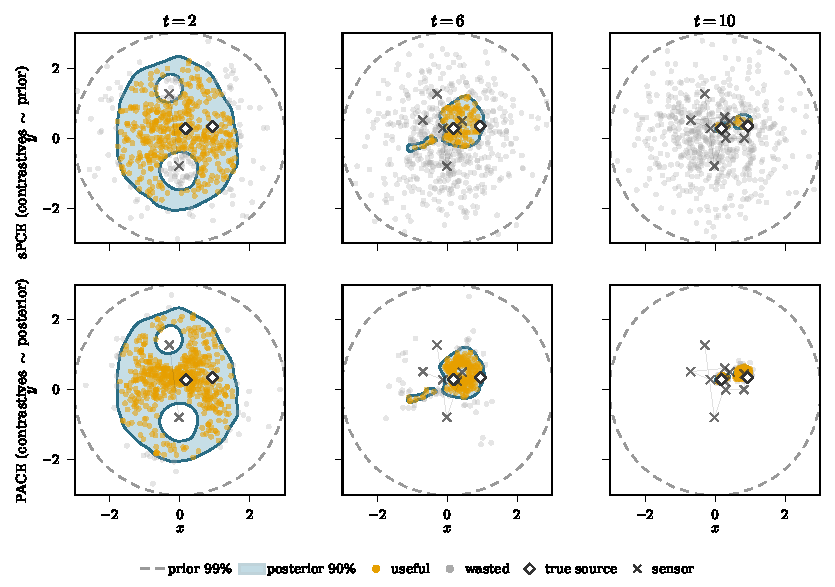
\includegraphics[width=0.8\linewidth]{figures/fig_a1_contraction.pdf}
  \caption[Posterior contraction and ESS collapse]{Posterior contraction and
  effective sample size across BED steps. As the posterior concentrates, the
  proposal mismatch grows and the ESS collapses, yet the per-step information
  $\Delta S_t$ remains positive and the design ranking is preserved.}
  \label{fig:contraction}
\end{figure}

\section{Design selection under weight collapse}
\label{sec:m-lowess}

This section answers RQ3. We derive a decomposition of the PACE score that separates a
design-independent part from the part that ranks designs, show that the collapsing
weight scale enters only the design-independent part, and identify the limiting
criterion.

\subsection{Decomposition into weight entropy and a design-dependent term}
\label{sec:m-decomp}

Define the cross-particle likelihood ratio
$r_{k\leftarrow j}(\xi_t)=p(y_{t,j}\mid\theta_k,\xi_t)/p(y_{t,j}\mid\theta_j,\xi_t)$,
with $r_{j\leftarrow j}=1$, and the competitor ratio
$\Psi_j(\xi_t)=\sum_{k\ne j}(w_k/w_j)\,r_{k\leftarrow j}(\xi_t)$. Starting from
Eq.~\eqref{eq:pace}, substitute $\tilde w_k=w_k/W$ with $W=\sum_k w_k$ and factor
$p(y_{t,j}\mid\theta_j,\xi_t)$ out of the inner sum. For the $j$-th term,
\[
\log p(y_{t,j}\mid\theta_j,\xi_t)-\log\!\sum_k w_k\,p(y_{t,j}\mid\theta_k,\xi_t)+\log W
= \log W-\log w_j-\log\!\big[1+\Psi_j(\xi_t)\big],
\]
where the likelihood of the generating particle cancels and the $k{=}j$ term is split
off using $r_{j\leftarrow j}=1$. Taking the weighted sum over $j$ and using
$\sum_j\tilde w_j\log w_j=\sum_j\tilde w_j\log\tilde w_j+\log W=-H(\tilde w)+\log W$,
the $\log W$ terms cancel and
\begin{equation}
\label{eq:decomp}
\hat I^{\mathrm{PACE}}(\xi_t)
= \underbrace{H(\tilde w)}_{\text{constant in }\xi_t}
- \underbrace{\sum_j \tilde w_j\log\big[1+\Psi_j(\xi_t)\big]}_{\bar\Phi(\xi_t)},
\end{equation}
with $H(\tilde w)=-\sum_j\tilde w_j\log\tilde w_j$ the entropy of the weights. The
weight entropy does not depend on the design, so
\begin{equation}
\label{eq:argmax}
\arg\max_{\xi_t}\hat I^{\mathrm{PACE}}(\xi_t)=\arg\min_{\xi_t}\bar\Phi(\xi_t).
\end{equation}

\subsection{The collapsed-weight limit}
\label{sec:m-collapse}

Now take the limit $\mathrm{ESS}\to1$, in which one weight dominates,
$\tilde w_{\mathrm{dom}}\to1$ and $\tilde w_j\to0$ for $j\ne\mathrm{dom}$. The
design-dependent term reduces to a single summand,
$\bar\Phi(\xi_t)\to\log[1+\Psi_{\mathrm{dom}}(\xi_t)]$. Since $\tilde w_{\mathrm{dom}}\to1$
forces $w_k/w_{\mathrm{dom}}\to0$ for every other $k$, we have
$\Psi_{\mathrm{dom}}(\xi_t)\to0$. Because $x\mapsto\log(1+x)$ is increasing,
$\arg\min_{\xi_t}\log[1+\Psi_{\mathrm{dom}}]=\arg\min_{\xi_t}\Psi_{\mathrm{dom}}$ holds
exactly, and the first-order expansion $\log(1+x)\approx x$ gives the interpretable
criterion
\begin{equation}
\label{eq:lr-limit}
\arg\max_{\xi_t}\hat I^{\mathrm{PACE}}(\xi_t)
= \arg\min_{\xi_t}\sum_{k\ne\mathrm{dom}}\frac{w_k}{w_{\mathrm{dom}}}\,r_{k\leftarrow\mathrm{dom}}(\xi_t).
\end{equation}
PACE selects the design that best separates the dominant particle from its
competitors, with fixed weights $w_k/w_{\mathrm{dom}}$. The monotone identity
$\arg\min_{\xi_t}\log[1+\Psi_{\mathrm{dom}}]=\arg\min_{\xi_t}\Psi_{\mathrm{dom}}$ is exact
for a single realised $y_{t,\mathrm{dom}}$; with $M{>}1$ observation draws per particle,
Algorithm~\ref{alg:ftk} ranks designs by the mean of $\log[1+\Psi_{\mathrm{dom}}(\xi_t)]$
over draws, which is the faithful scored objective and reduces to the weighted-ratio
form of Eq.~\eqref{eq:lr-limit} only at $M{=}1$.

\subsection{Common-mode cancellation}
\label{sec:m-cancellation}

Equation~\eqref{eq:lr-limit} is the validity argument. Under a collapsed weight set the
unnormalized weights can be astronomically large, which makes the PACE \emph{value} an
unreliable estimate of the EIG. The \emph{ranking} is protected for two reasons.
First, the weight entropy $H(\tilde w)$ in the decomposition~\eqref{eq:decomp} is
identical across candidate designs and drops out. Second, inside $\bar\Phi(\xi_t)$ the
weights $\tilde w_j$ and the ratios $w_k/w_j$ are fixed by the particle bank; only the
likelihood ratios $r_{k\leftarrow j}(\xi_t)$ change with the design. The diverging
weight scale therefore enters only design-independent terms and cancels in the
ranking. This guards the ranking against the weight scale; it does not reduce Monte
Carlo variance, which we measure directly in Chapter~\ref{sec:results}.

The two regimes are joined smoothly by the single estimator. When the effective
sample size is high, $\bar\Phi$ is a well-resolved weighted average and PACE
approximates the EIG with $O(1/J)$ bias. As the weights concentrate, $\bar\Phi$
deforms continuously into the single-particle form, with no threshold and no mode
switch. In that limit, if one competitor $\theta_{k^\ast}$ dominates the rest, the
criterion becomes a pairwise log likelihood-ratio test, and its expectation over the
generated $y_{t,\mathrm{dom}}$ is the Kullback-Leibler divergence between the two
predictive distributions,
\begin{equation}
\label{eq:kl}
\mathbb{E}_{y_{t,\mathrm{dom}}}\!\left[\log\frac{p(y_{t,\mathrm{dom}}\mid\theta_{\mathrm{dom}},\xi_t)}{p(y_{t,\mathrm{dom}}\mid\theta_{k^\ast},\xi_t)}\right]
= D_{\mathrm{KL}}\!\big(p(y_t\mid\theta_{\mathrm{dom}},\xi_t)\,\|\,p(y_t\mid\theta_{k^\ast},\xi_t)\big).
\end{equation}
For Gaussian likelihoods with a linearised forward map, the two predictive means differ by
the design Jacobian acting on $\theta_{\mathrm{dom}}-\theta_{k^\ast}$, so the Gaussian KL of
Eq.~\eqref{eq:kl} reduces to the quadratic form
$\tfrac12(\theta_{\mathrm{dom}}-\theta_{k^\ast})^\top F(\xi_t)(\theta_{\mathrm{dom}}-\theta_{k^\ast})$,
where $F(\xi_t)$ is the Fisher information of the design. Treating $\theta_{k^\ast}$ as a
posterior draw with covariance $\Sigma_{\mathrm{post}}$ and taking the expectation over it
gives, through $\mathbb{E}[(\theta_{\mathrm{dom}}-\theta_{k^\ast})(\theta_{\mathrm{dom}}-\theta_{k^\ast})^\top]=\Sigma_{\mathrm{post}}$
(which holds exactly when $\theta_{\mathrm{dom}}$ equals the posterior mean; in practice
the dominant particle approximates the mode, so this step is a Laplace-level approximation),
the expected criterion
$\tfrac12\,\mathrm{tr}\!\big(F(\xi_t)\Sigma_{\mathrm{post}}\big)$: Fisher information weighted
by residual posterior uncertainty, which is the D-optimal and classical Fisher design
objective of Section~\ref{sec:rw-classical}. This is the trace form of the
Gaussian-linearised EIG, so the quantity $\Lambda$ that drove saturation in
Section~\ref{sec:m-saturation} reappears here as the design objective; the underlying Laplace
linearisation is derived in full in Appendix~\ref{app:lindley}.

\subsection{Failure modes}
\label{sec:m-failure}

Two situations make the criterion uninformative. If the parameter differences between
the dominant particle and its competitors lie in directions that no design can
resolve, that is in or near the null space of $F(\xi_t)$ for all competitors and all
candidate designs, then Eq.~\eqref{eq:lr-limit} is flat and carries only noise.
Maximising a flat, noisy criterion can do slightly worse than uniform sampling, which
at least spreads coverage. This is an identifiability plateau, and the Goodwin
oscillator in Chapter~\ref{sec:results} is an example. Separately, if the NPE places
its mass in a region disjoint from the true posterior, the dominant particle is far
from the truth and PACE optimises designs to separate wrong hypotheses from each
other. This mode collapse is detectable through the diagnostics of
Section~\ref{sec:m-eval} (a diverging Pareto shape of the weights, raw coverage going
to zero), and we find no evidence of it on our systems, which is expected for the
unimodal posteriors of well-observed ODE systems.

\section{Forward-only design optimisation}
\label{sec:m-forward}

The reason to pair PACE with a forward-only optimiser is the same reason policy
training is expensive on the systems that motivate this work. A policy gradient
differentiates the sPCE objective with respect to the design, and therefore through
the simulator, by an adjoint pass. Each training iteration simulates $L$ contrastive
trajectories of $T$ steps forward and then backpropagates through all $L\cdot T$
solves. On stiff systems the backward pass is substantially more expensive than the
forward pass and carries a large fixed adjoint-compilation overhead~\citep{kim2024stiff,pal2023neural,caldana2025neural}.
Moreover, on saturated systems $L$ must reach $L_{\mathrm{escape},50}$ before the
gradient carries any signal at all (Section~\ref{sec:m-saturation}), so the total
training cost is $O(N_{\mathrm{iter}}\cdot L_{\mathrm{escape},50}\cdot T)$
forward-plus-backward solve pairs. For SEIR R=3, with $L_{\mathrm{escape},50}>10^6$ and
$T=10$, this exceeds $10^{10}$ solve pairs; for ASM1, with $L_{\mathrm{escape},50}\sim10^4$
and a stiff integrator, the adjoint overhead makes policy training infeasible in our
infrastructure. PACE removes the backward pass entirely. The NPE is trained without
differentiating through the simulator, and at deployment designs are chosen by search.

\subsection{Forward-only search}
\label{sec:m-ftk}

Algorithm~\ref{alg:ftk} draws the particle bank once per step, samples candidate
designs, scores each with PACE, and optionally refines the pool with one or more
cross-entropy rounds~\citep{rubinstein2004cross}. The per-step cost is
$J\big(1+M(1+C)N_{\mathrm{cand}}\big)$ forward solves: $J$ to weight the particles
against the history once, and $M$ observation draws for each of the
$(1+C)N_{\mathrm{cand}}$ scored candidates. There is no backward pass and no
differentiable simulator, so the method applies to stiff and black-box simulators.
Common-mode cancellation (Section~\ref{sec:m-cancellation}) guarantees that the search
optimises the correct ranking even when the effective sample size has collapsed.

\begin{algorithm}[t]
\caption{Forward-only design search (PACE-ftk) at step $t$}
\label{alg:ftk}
\begin{algorithmic}[1]
\Require history $h_{t-1}$, NPE $q_\phi$, particles $J$, draws $M$, candidates
$N_{\mathrm{cand}}$, rounds $C$, elite fraction $\rho$
\State draw $\theta_{1:J}\sim q_\phi(\theta\mid h_{t-1})$ and compute
$\tilde w_{1:J}$ by Eq.~\eqref{eq:weights}
\State sample $\{\xi^{(k)}\}_{k=1}^{N_{\mathrm{cand}}}\sim\mathrm{Uniform}(\Xi)$
\For{$k=1,\dots,N_{\mathrm{cand}}$}
  \State score $\hat I^{(k)}\gets\frac1M\sum_{m=1}^{M}\hat I^{\mathrm{PACE}}(\xi^{(k)})$ by Eq.~\eqref{eq:pace} \Comment{$JM$ forward solves}
\EndFor
\For{$c=1,\dots,C$}
  \State fit a Gaussian to the top $\lceil\rho N_{\mathrm{cand}}\rceil$ designs; resample $N_{\mathrm{cand}}$, clip to $\Xi$, rescore
\EndFor
\State \Return the best-scoring design over the whole pool
\end{algorithmic}
\end{algorithm}

\subsection{Gradient variant}
\label{sec:m-grad}

On systems where the simulator gradient is reliable, the PACE score can also be
optimised by gradient ascent. We call this variant PACE-grad
(Algorithm~\ref{alg:grad}). It differs from a policy method in a crucial way: it
differentiates through the simulator only at \emph{deployment}, to refine a single
design, not during a costly training loop, and it never relies on the saturated sPCE
signal. It warm-starts from the best of $N_{\mathrm{cand}}$ random candidates and runs
a few Adam steps from each of $R$ restarts. We include it to separate the contribution
of the estimator from that of the optimiser: PACE-ftk and PACE-grad share the same
one-time NPE proposal and candidate budget, so comparing them isolates the optimiser
(Chapter~\ref{sec:results}). Gradient ascent helps where the gradient is informative
and hurts on stiff systems where it is not, which is the empirical case for the
forward-only default.

\begin{algorithm}[t]
\caption{Gradient design search (PACE-grad) at step $t$}
\label{alg:grad}
\begin{algorithmic}[1]
\Require history $h_{t-1}$, NPE $q_\phi$, particles $J$, draws $M$, warm pool
$N_{\mathrm{cand}}$, restarts $R$, Adam steps $K$, step size $\eta$
\State draw $\theta_{1:J}\sim q_\phi(\theta\mid h_{t-1})$ and compute $\tilde w_{1:J}$
\State sample $N_{\mathrm{cand}}$ candidates, score by Eq.~\eqref{eq:pace}, keep the top $R$ as warm starts $\{\xi^{(r)}_0\}$
\For{$r=1,\dots,R$}
  \For{$k=1,\dots,K$}
    \State $\xi^{(r)}_{k}\gets\mathrm{clip}_\Xi\!\big(\xi^{(r)}_{k-1}+\eta\,\nabla_{\xi}\,\tfrac1M\textstyle\sum_m\hat I^{\mathrm{PACE}}(\xi^{(r)}_{k-1})\big)$ \Comment{adjoint through the simulator}
  \EndFor
\EndFor
\State \Return the best-scoring design among $\{\xi^{(r)}_{K}\}_{r=1}^{R}$
\end{algorithmic}
\end{algorithm}

\section{Evaluation protocol}
\label{sec:m-eval}

We evaluate every method on the same prior-contrastive scale. For each rollout we
report the bracket $[\mathrm{sPCE}_L,\mathrm{sNMC}_L]$, computed on the same rollouts
at the same $L$, which bounds the true mean EIG from below and above. These estimators
use the prior $p(\theta)$ in their denominator, so they bound the prior-contrastive
per-step gain, the common, method-agnostic scale shared by PACE, DAD, and random and
the one on which the saturation analysis operates. This is not the posterior-conditional
per-step EIG of Eq.~\eqref{eq:step-eig} that PACE's own estimator targets; the two
coincide at $t{=}1$ (empty history) and are reconciled step by step by the chain-rule
increments $\Delta S_t$ introduced below. When one method's lower bound exceeds
another's upper bound by more than the combined standard error, the ordering is
definitive and no estimation slack can reverse it. All main
comparisons use $n=300$ paired rollouts, three data-generating seeds of one hundred
each, with paired tests, since small-sample sPCE estimates are unreliable.

To see where information is acquired within a rollout, we also report the per-step
increment $\Delta S_t=S_t-S_{t-1}$, where $S_t$ is the sPCE on the length-$t$ prefix.
These increments telescope to the trajectory sPCE (Appendix~\ref{app:background}) and
show how much each step contributes as the posterior contracts. Because PACE is
deployed with a collapsing effective sample size, we report four diagnostics that each
rule out a specific failure: bootstrap pick-stability, raw versus importance-resampled
posterior coverage, per-step simulation-based calibration, and the Pareto shape of the
weights. These are developed with the results in Chapter~\ref{sec:results} and in full
in Appendix~\ref{app:diagnostics}. The suite of twelve systems is specified in
Appendix~\ref{app:systems}.

\section{Synthesis: one quantity, four roles}
\label{sec:m-synthesis}

The four results are linked by the likelihood ratio $r$ and its prior average
$e^{-\Lambda}$. In Section~\ref{sec:m-saturation}, $\mathbb{E}[r]\sim e^{-\Lambda}$ is
what drives sPCE to its ceiling, vanishes its gradient, and makes the escape budget
grow as $e^{\Lambda}$. In Section~\ref{sec:m-pace}, the same concentration that shrinks
$\mathbb{E}[r]$ reappears as the chi-square divergence in Eq.~\eqref{eq:ess} and
collapses the effective sample size; PACE removes the saturation but inherits this as
the cost of amortized inference. In Section~\ref{sec:m-lowess}, under that collapse the
design criterion reduces to a weighted sum of the same ratios $r$
(Eq.~\eqref{eq:lr-limit}) and approaches the Fisher value $\Lambda$ in a new role, now
the objective rather than the obstacle (Eq.~\eqref{eq:kl}). Chapter~\ref{sec:results}
closes the loop: the crossover between PACE and the policy is predicted by the
saturation threshold, the $\Lambda$ side of this object, and not by the effective
sample size, the chi-square side. One quantity therefore explains why prior
contrastives fail, how PACE fixes it, why the fix stays valid under its own cost, and
when the method wins.
